\chapter{Introduzione}
\label{chap:intro}

L'obiettivo di questo documento consiste nell'esposizione del lavoro svolto durante il periodo di Stage++ in Loccioni. Le competenze apprese spaziano tra know-how che caratterizza l'impresa e i suoi collaboratori, le capacità organizzative che derivano dal lavorare in un team e, naturalmente, nelle tecnologie utilizzate e l'architettura sviluppata.
Stilare report settimanali ci ha consentito di tracciare con precisione i progressi del nostro progetto, oltre che a poterci confrontare con esperti per poter garantire uno sviluppo regolare e senza errori di sorta.
Una caratteristica che spicca nel far parte di questo ambiente è quella della collaborazione orizzontale, dove noi studenti abbiamo percepito l'importanza attribuitaci: tutto ciò ha comportato un'esperienza di valore, dove le conoscenze apprese negli studi sono state sfruttate ed integrate completamente.
Questo ci ha consentito peraltro di avere un rapporto diretto con sviluppatori altamente qualificati, altrimenti impossibile in altre realtà dove una divisione del lavoro verticale implicherebbe una minore integrazione dei tirocinanti.
Poter prender parte allo stage anche nel periodo in cui l'emergenza sanitaria dovuta al COVID-19 costringeva al lavoro da remoto è stato estremamente valido a livello formativo. Sebbene alcune attività fossero impossibili da attuare, l'esperienza di apprendimento non si è mai fermata, garantendo in pieno la continuità del tirocinio.
Quello che Loccioni pone al centro della sua value proposition si può riassumere in una frase riportata nel sito dell'impresa stessa: "Trasformiamo i dati in valore" \cite{Loccioni}.
La sua principale attività è quella di progettare e realizzare sistemi di misura per 
testare e controllare componenti di auto, lavatrici ed altri strumenti elettronici.
Queste mansioni sono svolte in "linee di test"; ogni "linea" è strutturata in più "banchi" che a loro volta sono composti da più "stazioni", all'interno delle quali avviene 
il test effettivo del pezzo, o del DuT (device under test).\\
I risultati dei test sono poi visualizzabili tramite widget all'interno di dashboard remote, prendendo i dati da un server centrale, 
o collocate in prossimità della macchina.
\begin{figure}[h!]
\begin{center}
  
\includegraphics[width=10cm]{images/loccioni.jpg}
 \caption{Loccioni}
\end{center}
\end{figure}

\pagebreak
Nelle figure sottostanti sono raffigurati dei \textit{Banchi di Prova} per il testing di componenti. In entrambe la immagini è possibile osservare un pannello di controllo impiegato per la visualizzazione dei dati derivanti dai test effettuati sui componenti.
\begin{figure}[h!]
\begin{center}
  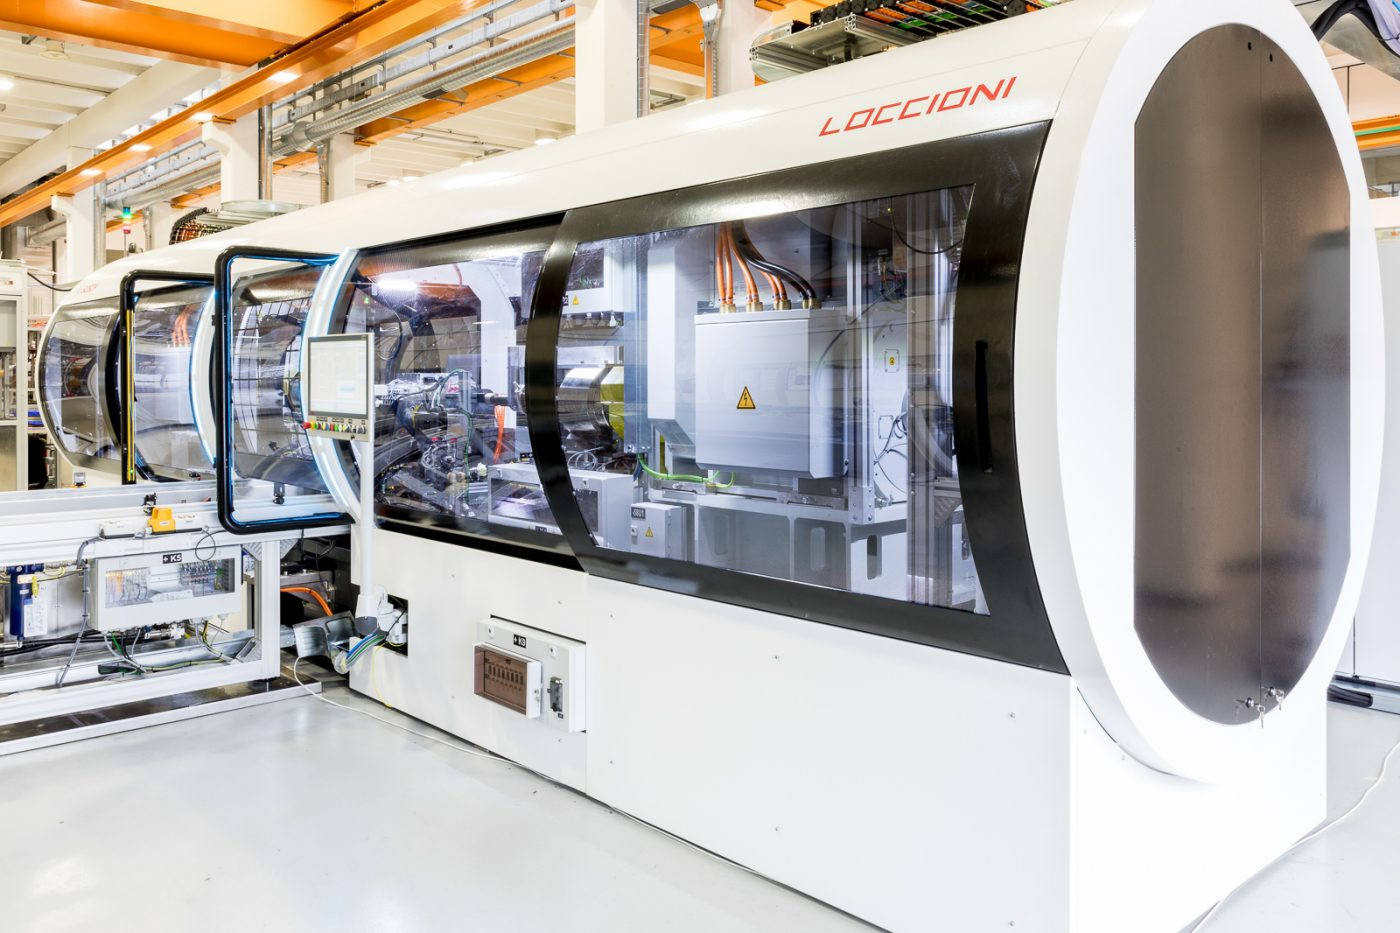
\includegraphics[width=15cm]{images/banco.jpg}
 \caption{Esempio di banco Loccioni}
 \label{fig:bancoLoccioni}
\end{center}
\end{figure}
\begin{figure}[h!]
\begin{center}
  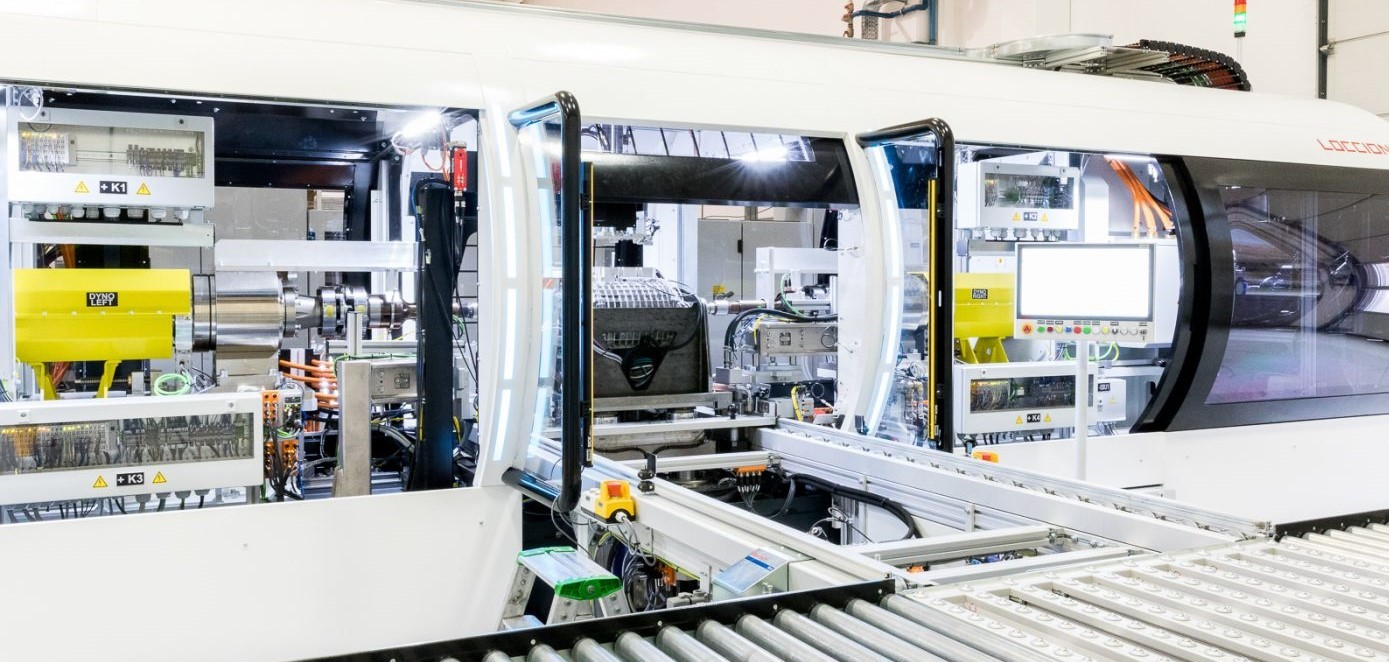
\includegraphics[width=15cm]{images/linea.jpg}
 \caption{Esempio di banco Loccioni}
 \label{fig:dashLoccioni}
\end{center}
\end{figure}

\pagebreak
\section{Obiettivo}
Il proposito del progetto è stato quello di ideare e realizzare una sovrastruttura per il framework AULOS, che verrà approfondito nel capitolo~\ref{chap:aulos}, per agevolare e rendere più efficiente lo sviluppo dei widget. Punto focale per ottenere questo risultato è stato effettuare uno studio delle caratteristiche che accomunavano più widget tramite un processo di graduale generalizzazione.
Quello che ne risulta è la creazione stessa dei widget in questione, con caratteristiche di flessibilità ed adattabilità: sarà infatti facilitato il ritrovamento dei dati dello stesso formato provenienti da fonti diverse. \\
Una lista di widget realizzati per lo studio sopracitato è presente nel capitolo~\ref{chap:widget}.

\section{Articolazione Tesi}
L'esposizione di questo elaborato sarà così suddivisa:
\begin{itemize}
    \item Il capitolo \ref{ch:metodologia} descrive le modalità di svolgimento del lavoro relativo al progetto, in particolare riguarda l'organizzazione interna del team
    \item Il capitolo \ref{chap:tecnologie_strumenti} in cui vengono indicate e dettagliare le tecnologie e gli strumenti utilizzati nel corso del progetto, approfondendo in particolare ciò che è stato impiegato nello sviluppo dell'applicativo backend e frontend
    \item Il capitolo \ref{ch:architettura} relativo all'organizzazione architetturale, specificando nel dettaglio tutte le parti che compongono il progetto
    \item Il capitolo \ref{ch:stresstesting} volto ad esporre le statistiche di performance raccolte in seguito allo svolgimento dei test di carico
    \item Il capitolo \ref{chap:conclusione} che conclude la tesi presentando un sunto del lavoro svolto e sottolineando i punti salienti che sono stati raggiunti, vengono inoltre accennati possibili futuri sviluppi del sistema
\end{itemize}